%% FAIR'2026 submission -- draft
%% Template: IEEE conference (IEEEtran). Limit: 8 pages, max 5 keywords.
%% STATUS: Section VII reports the status of the model study. No executability
%%         score exists for any trained branch. Do not fill Table VI with estimates.
\documentclass[conference]{IEEEtran}
\IEEEoverridecommandlockouts

% IEEE conference proceedings require Times/Helvetica/Courier. Under XeTeX the
% legacy ptm/phv/pcr shapes do not resolve, so we load the metric-compatible
% TeX Gyre family explicitly; Termes also carries the Vietnamese diacritics
% needed for the author names.
\usepackage{fontspec}
\setmainfont{texgyretermes}[
  Extension = .otf, UprightFont = *-regular, BoldFont = *-bold,
  ItalicFont = *-italic, BoldItalicFont = *-bolditalic ]
\setsansfont{texgyreheros}[
  Extension = .otf, UprightFont = *-regular, BoldFont = *-bold,
  ItalicFont = *-italic, BoldItalicFont = *-bolditalic ]
\setmonofont{texgyrecursor}[
  Extension = .otf, UprightFont = *-regular, BoldFont = *-bold,
  ItalicFont = *-italic, BoldItalicFont = *-bolditalic, Scale = MatchLowercase ]
\usepackage{cite}
\usepackage{amsmath}
\usepackage{unicode-math}
\setmathfont{texgyretermes-math.otf}   % Times math, matches the body text
\usepackage{graphicx}
\usepackage{booktabs}
\usepackage{array}
\usepackage{pgfplots}
\pgfplotsset{compat=1.16}
\usepackage{url}
\usepackage[hidelinks]{hyperref}

\newcommand{\pend}{\textemdash}
% Termes carries no U+2713; spell the verdicts instead of risking a dropped glyph.
\newcommand{\vpass}{\textsc{pass}}
\newcommand{\vfail}{\textbf{\textsc{fail}}}

\begin{document}

\title{Executability: A Reference-Free Metric for\\
Element Identification in Generated GUI Instructions}

\author{\IEEEauthorblockN{Lê Đoàn Phương Uyên}
\IEEEauthorblockA{\textit{Faculty of Information Technology} \\
\textit{University of Science, VNU-HCM}\\
Ho Chi Minh City, Vietnam \\
24C15039@student.hcmus.edu.vn}
\and
\IEEEauthorblockN{Nguyễn Hồng Bửu Long}
\IEEEauthorblockA{\textit{Faculty of Information Technology} \\
\textit{University of Science, VNU-HCM}\\
Ho Chi Minh City, Vietnam \\
nhblong@fit.hcmus.edu.vn}
}

\maketitle

\begin{abstract}
GUI agents produce coordinates for a machine to click. We study a different output: a
short instruction telling a person which on-screen element to touch. We ask a narrower question than ``is this a
good instruction'': only whether the sentence identifies the right element. Many
wordings do, so no single reference can carry the judgement: scored against one,
$53\%$ of the sentences our metric accepts from an untuned model fall below a
lenient overlap threshold against $14\%$ for a fine-tuned one, so the penalty falls
unevenly between systems. We propose \emph{executability}: the sentence goes to a separate GUI grounding
model that never sees the gold coordinate, and a step counts as
correct when the returned point falls in the cell of the element the user touched
and the described action matches. This paper characterises that instrument on
AndroidControl. The grounder attains a median localisation error of $0.7\%$ of
screen width against a threshold of $3\%$ fixed in advance. The hit rule is chosen on
its measured floor: the conventional tolerance test credits a sentence naming the
wrong button in $84.3\%$ of cases, the cell rule in $2.8\%$. Human-written references
score $75.7\%$ (95\% CI $[74.1, 77.3]$), the level every model score has to be read
against, and a contentless sentence scores $12.0\%$, fixing the other end of the scale;
a genuine sentence written for a different screen scores lower still, $6.1\%$. Removing
the element name from a reference costs $28.5$ points where removing the locative clause
costs $3.5$, so the measurement is dominated by naming rather than by pointing. The supervision behind the study is built automatically from $64{,}567$
steps with no task leakage. Applied over $4{,}462$ held-out steps to a QLoRA-tuned
Qwen2.5-VL-3B at two seeds and to the same model untuned, the metric returns $59.4\%$
and $47.6\%$; the paired gap of $11.8$ points survives six checks for alternative
explanations, among them one discarding every sentence that reproduces the reference
word for word. Retraining the same design under a different seed moves the score by
$0.5$ points, so the effect stands at $22\times$ the metric's retraining noise, and the
instrument itself contributes none of that variance: identical sentences return
identical verdicts. We also report what the metric cannot do, including a contamination
path we cannot close with the grounder in hand.
\end{abstract}

\begin{IEEEkeywords}
GUI instruction generation, vision-language models, reference-free evaluation,
AndroidControl, pre-registration
\end{IEEEkeywords}

\section{Introduction}

Given a mobile screenshot and a user goal, a GUI agent predicts an action such as
\texttt{click(872,141)}. A different consumer of the same input is a person who
needs to be told what to do: \emph{tap the pencil icon at the top right of the
note}. Systems serving this second consumer are appearing in accessibility and user-support
settings~\cite{guideme}, but the generation problem has had little quantitative
treatment.

The obstacle is evaluation. A recorded touch coordinate can be compared with a
predicted one; a sentence cannot be compared with a single reference, because many
wordings identify the same button and no dataset enumerates them.
The GUI agent literature does not resolve this. In Aguvis~\cite{aguvis} the model emits a low-level
natural-language instruction, but only as an intermediate representation en route to
an action, and its quality is never scored.
In the AndroidControl corpus~\cite{androidcontrol} the human-written per-step
instruction is an \emph{input} that conditions action prediction. In the present
work it is the generation target and the only scored output.

We therefore treat measurement as the primary object of study. Our metric,
\emph{executability}, closes the loop through a third party: the sentence goes to a
separate grounding model~\cite{uground}, and the step counts as correct if that model
locates the element the user touched. The term is used differently
in open grounded planning~\cite{ogp}, where executability is the share of plans whose every
action appears in a given action library --- a symbolic lookup over text. Ours is
behavioural and visual: a model reads the sentence, looks at the screen, and points. Two lines of work meet here. Referring-expression
generation judges a description by whether a listener resolves
it~\cite{mao2016,luo2017,yu2017}; reference-free hallucination detection verifies
claims against an external source rather than the generator's own
beliefs~\cite{aloha}. Whether such a metric is dependable enough to support a
conclusion is an empirical question, and most of this paper answers it.

The intervention we intend to evaluate with it is a training-target modification: a 3B
vision--language model~\cite{qwen25vl} fine-tuned with QLoRA~\cite{lora,qlora} emits a
structured descriptor of the target element before the sentence, and the descriptor is
removed before scoring. We claim no novelty for the idea, the core of
referring-expression generation since 2016~\cite{mao2016,luo2017,yu2017}; supplying
element lists as input is likewise standard~\cite{androidcontrol,mind2web,widgetcap}.
The untested question is whether it transfers to GUI instructions, and whether it
survives a length-matched false descriptor and one with the coordinate removed.

The contributions of this paper are:

\begin{enumerate}
\item an executability metric for element identification in GUI instructions, with
the hit rule selected from measured behaviour on wrong-element inputs rather than on
tolerance, and shown to preserve the ordering of systems under five different rules
(Section~\ref{sec:metric});
\item a characterisation of the instrument: an adequacy gate on grounder error, a
measured ceiling of $75.7\%$, a sensitivity curve on the deployed grounder, a
validation by controlled error injection against thresholds fixed in advance, and
a measurement of what a reference-based score would have concluded on the same
sentences (Sections~\ref{sec:gate}--\ref{sec:inject});
\item a fully automatic pipeline converting AndroidControl into supervision for this
task, with coverage, invariants and leakage verified at full scale
(Section~\ref{sec:data});
\item a pre-registered ablation design with the decision rule for all four outcomes,
committed to version control before the first training run
(Section~\ref{sec:design});
\item an application of the instrument to a fine-tuned 3B model at two seeds, which
places two real systems against the ceiling, measures the metric's own retraining
noise floor, and localises where the remaining error lies (Section~\ref{sec:status}).
\end{enumerate}

The ablation itself is still running; we report the baseline arm and the diagnostics
it supports, and leave the comparison rows of Table~\ref{tab:main} empty.

\section{Related Work}

\subsection{GUI grounding, agents, and element lists}
AndroidControl~\cite{androidcontrol} provides $15{,}283$ human-recorded episodes with
per-step instructions and gold touch coordinates; AndroidInTheWild~\cite{aitw} is the
source of the $14\%$ tolerance convention. Grounding models such as SeeClick~\cite{seeclick},
OS-Atlas~\cite{osatlas} and UGround~\cite{uground} map a text expression to a screen
point; we use one as an instrument, not a baseline, and report its measured error and
training mixture before depending on it.

Supplying a structured list of screen elements is likewise established: the
AndroidControl authors fine-tune with an accessibility-derived element list as input
and state that their agent does not use the screenshot~\cite{androidcontrol},
Mind2Web~\cite{mind2web} trains over noisy candidates, and Widget
Captioning~\cite{widgetcap} puts the view hierarchy at the input. We make no
contribution claim for this layer; it appears only as an ablation branch.

\subsection{Discriminative description generation}
Producing a description that identifies one object among distractors is the
referring-expression generation task~\cite{mao2016}, and later work places a
comprehension model inside the training loop to enforce
discriminativeness~\cite{luo2017,yu2017}. The closest supervised work in the GUI domain
is Widget Captioning~\cite{widgetcap}, which identifies the problem of visually
identical widgets but trains with plain cross-entropy. Our target is narrow
accordingly: discriminativeness in the training target for GUI instructions.

\subsection{Reference-free evaluation}
Verifying generated text against an external structured source rather than the
generator's own beliefs is the principle behind ALOHa~\cite{aloha}, and perturbation
checklists with pre-declared thresholds are an established way of validating a
metric~\cite{sai2021}. One difference matters: ALOHa checks against a static list, we
check against a learned model, a weaker guarantee. Two cautions apply directly, that
automatic proxies for human judgement are easily over-trusted~\cite{clark2021} and
that grounder accuracy measured on one ``best'' instruction per element overstates
what these models can do~\cite{groundersunderstand}; both return in
Section~\ref{sec:limits}.

\section{Task Definition and Dataset Construction}
\label{sec:data}

The task is: given one screenshot $I$ and a user goal $q$, produce a single
instruction $s$ in natural language identifying the element to be touched and the
action to perform, addressed to a human reader.

\subsection{Sources and cross-modal alignment}
Three ingredients are required per step: the human-written instruction, the
screenshot, and an accessibility tree. No single public redistribution of
AndroidControl~\cite{androidcontrol} carries all three, so we join two
Hugging Face mirrors on \texttt{(episode\_id, step\_id)} and take accessibility
trees for $99{,}131$ screens from the same release.

One property of the redistribution has to be stated: goal strings are truncated at
source, $99.0\%$ ending mid-phrase (\texttt{...look for Calvin Kle}). Every trained arm
reads the same truncated goal, so it cannot explain a difference between them, but the
reference arm sees no goal at all, so the model-to-reference distance is to that extent
an over-estimate.

An off-by-one join would corrupt every downstream label while leaving the pipeline
functional, so we test it: OCR at the gold touch point should be found in the
reference instruction more often under the correct join than under a control shifted
by one step. On $n=400$ sampled steps it matches $48\%$ against $20\%$, intervals
that do not meet.

\subsection{Scale, splits and leakage}



The corpus holds $64{,}567$ training and $6{,}958$ test steps over $12{,}895$ and
$1{,}432$ tasks; about $64\%$ of each are touch steps and form the scoring population.
OCR covers every step with no image missing, descriptor labels cover $99.7\%$ of test
touch steps, and the split is held out by task with zero overlap, verified at full
scale since leakage cannot be repaired after training. Task disjointness is not phrase
disjointness: on a $1{,}697$-step slice of the training data, itself $2.6\%$ of it,
$17.3\%$ of test references already appear verbatim and $66.5\%$ share a 4-gram,
because the corpus reuses wordings such as \emph{click on the search bar}. The
reproduction check of Section~\ref{sec:status} removes sentences copied from their own
step; it cannot remove this.

Two properties of the split constrain what may be concluded. First, it is not held
out by application: $95.6\%$ of attributable applications also occur in training. The primary comparison is unaffected, since all branches share training
data, base model and test set, so a difference between two branches still isolates
the intervention; a comparison against an external model that never saw these
applications would carry a home-field advantage, and we report no such comparison as
a standalone result. The effect can now be bounded directly, since the fine-tuned
model scores $59.1\%$ on seen applications and $59.0\%$ on unseen ones
(Section~\ref{sec:status}). Second, only $45.0\%$ of test steps can be
attributed to a named application ($269$ applications); the remaining $3{,}828$
steps are labelled \emph{unknown}, which is distinct from \emph{unseen} and is
never read as such. This drives the clustering rule of Section~\ref{sec:power}.

\subsection{On-screen text extraction}
Accessibility trees are the natural source of element names, but across the
$99{,}131$ screens only $12.6\%$ of elements carry any name, consistent with
reports that most Android applications ship incomplete accessibility
labels~\cite{chen2020}. The available dump also contains developer-facing content
descriptions instead of displayed text. We therefore run OCR (RapidOCR, ONNX, CPU)
over every screenshot and use it both as an input feature and as a name source,
obtaining $64{,}567$ records with zero missing.

The stage was cross-checked between two machines five days apart, $24.2$ recognised
strings per screen on the test split against $23.6$ on training with identical medians.
AndroidControl has no text ground truth, so we make no accuracy claim. OCR fails two
ways: icons read as characters, and spaces swallowed (\texttt{Turnon}), the latter
pushing an element into the \emph{no name} bucket rather than assigning a wrong one.

\subsection{Automatic descriptor labels}
The training target of the treatment branch contains a structured descriptor built
without human annotation. From the gold touch coordinate we select the smallest
accessibility box containing it; the role is taken from the tree; the name comes
from the tree when it passes a validity gate, and otherwise from OCR inside the box;
the coordinate slot holds the gold touch point on a $[0,1000]$ grid; and a fourth
slot holds a distinguishing cue computed by rule.

Two gates were introduced on measured grounds: a validity gate rejecting $14.7\%$ of
accessibility labels at target nodes (source-code identifiers, long digit strings,
screen-reader suffixes, empty phrasings) and a geometric gate restricting OCR name
extraction to boxes under $25\%$ of the screen. The fourth slot needed revision: on a
pilot slice only $7.3\%$ of cues resolved anything, $85.8\%$ merely counting. Ordering
the rules by whether a clause resolves ambiguity and adding a text anchor, the nearest
OCR string outside the box with its direction, raised that to $75.9\%$.

At full scale ($41{,}191$ touch steps) $73.6\%$ of labels carry a clear name, $4.4\%$
a symbol only and $22.0\%$ no name; the $32{,}061$ names come $8{,}581$ from the tree
and $23{,}480$ from OCR. A same-role neighbour is present on $91.6\%$ of screens. Five reference quantities
agree with the pilot slice to within one point, so the builder did not degrade when
scaled by $24$.

\subsection{Branches and structural invariants}
Four datasets are built from identical inputs and differ only in the generation
target: \textbf{s1}, the sentence alone; \textbf{s2}, descriptor then sentence;
\textbf{s2r}, a false descriptor from a different screen with randomised
coordinates, token-length-matched per example; and \textbf{s2\_nopoint}, s2 without
the coordinate slot. Length matching uses the model's own tokeniser and places
$99.3\%$ of pairs within two tokens, matching the descriptor prefix rather than the
emitted sentence. A target in s2 reads \texttt{<desc>item | CATEGORIES | <point>127,238</point> | left
of the text "MEN"</desc>} followed by the same scored sentence as s1.

Nine invariants are checked after every rebuild and all nine hold at full scale: the
scored sentence is byte-identical across branches on all $64{,}567$ examples; s1
carries no descriptor and s2\_nopoint no coordinate; the three descriptor branches
carry the same $41{,}099$ labels and s2 differs from s2r exactly on them; the negative
descriptor never reuses the target coordinate; and non-touch steps carry an identical
target everywhere, the precondition for the do-no-harm check of
Section~\ref{sec:power}.

\section{The Executability Metric}
\label{sec:metric}

\subsection{Definition}
Let $s$ be the generated sentence with any descriptor removed, $I$ the screenshot,
$g$ the gold touch coordinate, and $E$ the set of accessibility elements on the
screen after merging elements whose centres lie within $24$\,dp. Let $G$ be a
grounding model, independent of the model under test and without access to $g$,
returning a point $p = G(I, s)$. The step is scored correct when all three
conditions hold:
\begin{enumerate}
\item[(i)] \emph{action}: the canonicalised action types of $s$ and of the
reference agree. Canonicalisation maps twelve surface verbs (tap, click, press,
select, choose, touch, open, launch, go, navigate, visit, view) to a single class,
because on a screen all of them denote the same touch; the classes that remain
distinct are touch, type, scroll, long-press and back. The scan is left-to-right
and \texttt{go} precedes \texttt{back}, so \emph{go back} canonicalises to touch; on
the touch population that costs $0.3$ points for S1 and $0.2$ for the untuned model,
and we leave it uncorrected rather than change a metric after seeing scores, while
the do-no-harm check on non-touch steps, not yet run, uses the corrected function;
\item[(ii)] \emph{polarity}: $s$ and the reference do not name opposite states of
the same control, checked against a hand-written table of nine toggle pairs
(on/off, enable/disable, show/hide, mute/unmute, expand/collapse, check/uncheck,
select/deselect, start/stop, enabled/disabled) after removing position words;
\item[(iii)] \emph{localisation}: $p$ lies within the conventional tolerance of the
gold point, $|p_x - g_x| \le \tau W$ and $|p_y - g_y| \le \tau H$ with $\tau =
0.14$ following~\cite{aitw}, \emph{and} no competing element centre is closer to
$p$ than $g$ itself: $\lVert p - g\rVert < \lVert p - c(e)\rVert$ for every
$e \in E$.
\end{enumerate}
Two details of (iii) are easy to state imprecisely. The tolerance region is a
rectangle taken per axis, as in~\cite{aitw}, not a disc: $\pm151$ px horizontally
and $\pm336$ px vertically on a $1080 \times 2400$ screen. And the site of the
target cell is the recorded touch point $g$, not the centre of the element
containing it, since $g$ is what the metric is accountable to; $E$ comes from the
accessibility tree with centres within $24$\,dp of $g$ removed, so a second box
belonging to the target does not compete with it. The rule refines the tolerance
test and never accepts a step that test rejects. Executability is the proportion of
touch steps satisfying all three conditions.

The rubric is a recorded human touch coordinate, not a model's opinion, so the design
is not LLM-as-judge: $G$ contributes a localisation and geometry against $g$ decides.
$G$ is never fine-tuned by us and never sees $g$, but it is no outsider. UGround-V1-2B is built on Qwen2-VL, the family of the model under test, and
its training mixture includes $47$K human-annotated elements from the AndroidControl
\emph{training} split~\cite{uground}; our test split is disjoint at the level of
screens, but the grounder has seen this corpus's annotation register, which
Section~\ref{sec:limits} treats as a live alternative explanation. The same $G$
scores every branch, removing any bias that acts equally on all of them, though not
one that tracks how closely a branch imitates that register --- and the arm imitating it most
closely is the reference arm, so the mechanism would lift the ceiling before any gap.
What the metric scores is narrow and worth naming: whether a sentence identifies the
right element, not whether a reader would find it a good instruction. Fluency, length
and usefulness lie outside it.

\subsection{Hit rule selection}

Is the nearest-element requirement needed on top of the conventional tolerance
test~\cite{aitw}? We compared three rules on $250$ touch steps, each measured twice: a
ceiling injecting a controlled offset into a perfect point, and a floor putting the
point on the nearest \emph{other} element, standing in for a sentence naming the wrong
button.

The floor decides it. Against a sentence naming the wrong button the tolerance test
still awards credit in $84.3\%$ of cases, a dynamic range of some $16$ points that
cannot separate a good instruction from a bad one; the cell rule awards $2.8\%$, a
range of about $97$ points, while holding a ceiling of $99.7\%$ under a $3\%$ offset.
Two caveats travel with that
floor. It covers sentences naming a \emph{distinct} element, not a point displaced
inside the target's own cell (Table~\ref{tab:inject}, row 4). And the merge defining
``distinct'' is not free: it deletes a competing centre on $96.3\%$ of steps, and on
$8.2\%$ at least one deleted centre belongs to a genuinely separate element. We report the tolerance
score alongside the headline, never as the headline.

\subsection{Grounder adequacy gate}
\label{sec:gate}
The metric inherits the reliability of $G$. Before committing compute we fixed a pass
condition of \emph{median localisation error at most $3\%$ of screen width}, derived
from screen geometry. Over $1{,}496$ touch steps the tolerance
margin, half the distance from the target to the nearest other element after
merging, has median $67$ px ($6.2\%$ of width) and 10th percentile $39$ px
($3.6\%$), so a $3\%$ threshold ($\approx 32$ px) sits below the 10th percentile.
The task is achievable in principle: AndroidControl touch coordinates are element
centres, $79.4\%$ within $1.5$ px of one.

UGround-V1-2B~\cite{uground} on $300$ test steps with a fixed seed attains a median
error of $0.7\%$ of screen width (p25 $0.2$, p75 $9.1$, p90 $36.3$; $62.7\%$ of
steps at or below $3\%$). The gate passes, but a median is a weak test on a
distribution this bimodal --- the grounder either lands near the centre or lands
elsewhere entirely --- and a percentile condition would have been the better choice.

Four installation-fault detectors were declared in advance and one fired: a horizontal
coordinate exactly at screen centre in $30.7\%$ of steps against a threshold of $20\%$.
Part is the data ($18.3\%$ of gold points are centred). The rest is not: among the
$245$ steps whose gold point is off centre the grounder answers at the centre $46$
times, in a band covering roughly $1\%$ of the axis. When it cannot identify an element
it abandons the horizontal axis. This depresses our scores rather than inflating them,
so the gate passes legitimately, but it is declared at every use of the metric.

\subsection{Metric ceiling}
\label{sec:ceiling}
The gate measures distance; the metric scores Voronoi cells. To obtain the highest
score the metric can award to a perfect generator, we passed the
\emph{human-written reference instruction} of every touch step to the grounder and
scored the returned points with the deployed hit rule. Over all $4{,}462$ touch
steps, $1{,}091$ clusters (effective $454.3$), the ceiling is $\mathbf{75.7\%}$
$[74.1, 77.3]$ under the Voronoi rule and $84.3\%$ $[82.9, 85.6]$ under the
tolerance test reported alongside it. That second figure coincides with the disk
floor of Section~\ref{sec:metric} to one decimal; the two are measured on different
populations and the agreement is accidental. Since the inputs are the references
themselves, conditions (i) and (ii) are satisfied on all but three steps, where the
polarity rule fires on a reference containing both ``on'' and ``off'', so the
ceiling is a localisation score to within $0.07\%$. Every executability figure must therefore be read against $75.7$ and
not $100$.

We call $75.7$ a ceiling and not a bound. It is the score of one particular class of
sentence, written by annotators for other people; a generator rewarded by this
metric could in principle exceed it by writing for the grounder instead, with
phrasings no reader asked for. Nothing in the construction forbids that, so an arm
approaching $75.7$ has to be read as a reason to inspect its sentences and not as a
success; the pre-registration halts the study in that case for a different reason,
namely that no room would be left to resolve (Section~\ref{sec:limits}).

An earlier estimate from the $300$ grounder outputs retained by the adequacy gate
gave $70.0\%$ $[64.5, 75.3]$, five points low and just outside its own interval: a
quantity that conditions every other number should not rest on a subsample.

\begin{figure}[t]
\centering
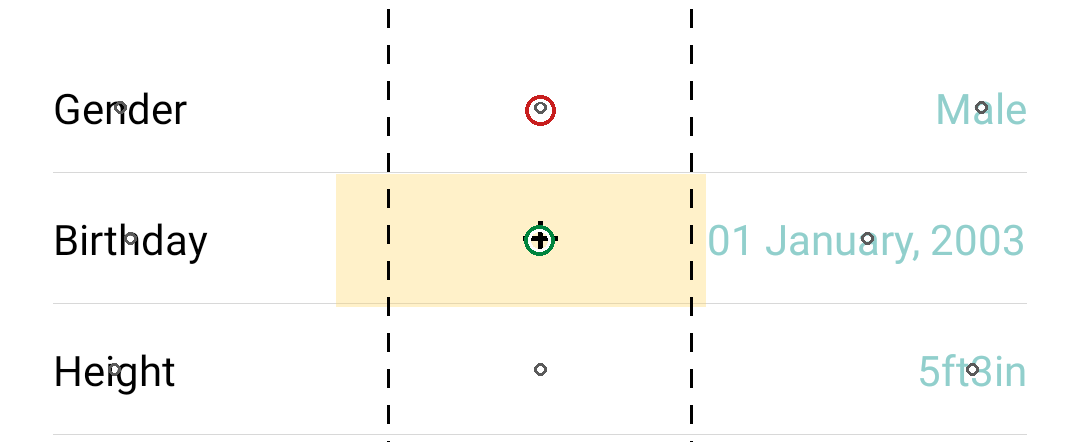
\includegraphics[width=0.78\columnwidth]{fig_voronoi.png}
\caption{Why the tolerance test alone cannot carry the judgement. The user touched the
\emph{Birthday} row; its cell is shaded and the fine-tuned model's sentence sends the
grounder to the cross inside it. The untuned model wrote ``Click on the `Gender'
section\ldots'' and the grounder went where it was told, $128$ px away on the row
above --- inside the $\pm336$ px vertical tolerance, so the conventional rule scores
it correct and the cell rule does not. Circles are competing element centres.}
\label{fig:cell}
\end{figure}

The same verdict holds on the deployed instrument: binning the $300$ gate steps by the
error the grounder actually made, the cell rule credits every step below the $3\%$
gate ($n=188$) and none above $14\%$ ($n=63$), while the tolerance test credits
everything up to $14\%$. Fig.~\ref{fig:cell} shows a step where they disagree.

Choosing a rule is a researcher degree of freedom, so we measured what the choice buys
and what it costs. Rescoring all three arms on $698$ steps under five rules --- a
Euclidean disc, the per-axis rectangle we use, the cell rule as implemented, a cell
rule seeded at the centre of the box containing $g$ instead of at $g$, and a
nearest-box rule --- gives ceilings of $80.2$, $82.2$, $74.2$, $56.6$ and $82.2$, and
S1 over the untuned model of $+12.6$, $+13.0$, $+11.7$, $+9.5$ and $+13.0$ points. The
absolute level moves by up to $26$ points, so no single value here is a property of the
systems alone. The ordering never moves, and the gap stays between $9.5$ and $13.0$
points, several times the detectable effect of Section~\ref{sec:power}.

\subsection{Validation by controlled error injection}
\label{sec:inject}

\begin{table}[t]
\caption{Metric self-check by injected errors. Thresholds fixed before execution.}
\label{tab:inject}
\centering
\footnotesize
\begin{tabular}{lrrrl}
\toprule
Criterion & Thr. & Obs. & $n$ & \\
\midrule
False reject, real paraphrase & $\le$10\% & 0.0\% & 398 & \vpass \\
False reject, action gate     & $\le$15\% & 0.0\% & 398 & \vpass \\
False reject, flip rule       & $\le$5\%  & 0.0\% & 398 & \vpass \\
Detect near neighbour         & $\ge$80\% & 33.1\% & 121 & \vfail \\
Detect far neighbour          & $\ge$90\% & 99.6\% & 233 & \vpass \\
Detect very far element       & $\ge$95\% & 100.0\% & 397 & \vpass \\
Detect held-out negation      & $\ge$50\% & 20.0\% & 15 & \vfail \\
Detect wrong action           & $\ge$80\% & 100.0\% & 369 & \vpass \\
Detect wrong content          & $\ge$90\% & 91.1\% & 494 & \vpass \\
Detect wrong direction        & $\ge$90\% & 100.0\% & 755 & \vpass \\
\bottomrule
\end{tabular}
\end{table}

Following the perturbation-checklist methodology~\cite{sai2021} we fixed ten criteria
and thresholds before execution ($398$ test touch steps). The aggregate ``8 of 10''
should not be read as an accuracy: five rows exercise a mapping against itself and
cannot fail by construction --- the action gate swaps verbs the canonicaliser calls
equivalent, the flip rule can fire only on three references, the wrong-action and
wrong-direction rows check a lookup against its own table, and the paraphrase row
injects its ``correct'' point $23$ px from the gold, inside the merge radius. Four
rows carry information, those placing the point on a neighbouring element or negating
the sentence, and two of the four fail.

The first failure follows from a design decision. The metric cannot distinguish
points displaced by less than approximately $63$ px, because the rule merges
elements whose centres lie within $24$\,dp ($63.1$ px at the $2.625$ density of a
$1080$-wide device). That radius
is just under the median tolerance margin of $67$ px reported in
Section~\ref{sec:gate}, so a displacement below it usually remains inside the
target's own cell. The metric therefore detects naming the wrong element and does not detect
pointing slightly off inside the correct one. The second failure concerns a thin
safety net for negation terms outside our lexicon and rests on $15$ cases, too few
to support a claim.

An earlier version of this self-check reported the same aggregate score with a
\emph{different} set of failures, because it scored with a hit function absent from
the deployed scoring path. The failure was silent: the program ran to completion and
produced plausible numbers for a metric other than the one in use.

\subsection{What a reference-based score would conclude}
\label{sec:refbased}
The premise that a single reference cannot carry the judgement is testable on the
sentences of Section~\ref{sec:status}. Scored with a content-word F1, $52.8\%$ of the
untuned model's accepted sentences fall below $0.5$ against $13.9\%$ for the fine-tuned
one: fine-tuning moves the wording towards the annotator's register, so the score
charges one arm more than the other for a property unrelated to identification.

Table~\ref{tab:main} carries BLEU-4 and ROUGE-L alongside for the same arms.
All three rank the arms alike. We draw nothing from that agreement: two measures can
agree and both be wrong about the property of interest, so concordance between them is
not evidence for either.
What it cannot do is say how much room is left: the reference arm scores $100$ on
ROUGE-L and $96.1$ on sentence-level BLEU-4, the shortfall being exactly the $176$
references shorter than four tokens, where executability measures $75.7$ and locates
the missing quarter. The two families also disagree about how far apart the models
are, by a margin that depends on the variant used, so the argument rests on the
unequal exposure ($52.8\%$ against $13.9\%$) and not on a ratio between scales.

\subsection{Secondary metric and statistical power}
\label{sec:power}
A mandatory do-no-harm check covers the $35.9\%$ of test steps that are not touch
steps: scrolling, waiting, typing, opening an application and going back. There the
treatment must not fall more than $3$ points below the control on action-type
agreement, computed with the canonicalisation function of the primary metric so that
a second and subtly different definition of action match cannot arise.

Confidence intervals use a nonparametric cluster bootstrap with $10{,}000$
resamples, clustered by application: whole clusters are drawn with replacement and
the interval is taken from the percentiles. Cameron et al.~\cite{cameron2008} show
this undercovers when clusters are few, which is why we report the cluster count
alongside every interval and treat the $G = 259$ restriction below with caution. The clustering rule determines the
available power and was therefore fixed in advance: steps that cannot be attributed
to an application form one cluster per task, giving $G = 1{,}091$ clusters and an
effective $G_{\text{eff}} = 454.3$ under Kish's formula~\cite{kish1965}, with the
largest cluster covering $58$ steps. The rule declines to assume that steps of
unrelated tasks which happen to lack an application label belong together, and the
result does not depend on it: the S1-over-Base interval is $[+10.0, +13.1]$ under
this rule, the same with every step clustered by task ($G = 1{,}345$), and
$[+10.2, +13.8]$ with all unlabelled steps forced into one cluster ($G = 260$).
Restricting the analysis to the $40.7\%$ of attributable steps gives $G = 259$ and
$G_{\text{eff}} = 107$. The projected minimum detectable effect
$2.8\,\hat{\sigma}/\sqrt{G_{\text{eff}}}$, where $2.8 \approx z_{0.975} + z_{0.80}$
gives $80\%$ power at the $5\%$ level, is
$3.9$--$6.6$ pp under the first rule and approximately $12.1$ pp under the second.
That formula divides by $\sqrt{G_{\text{eff}}}$, which assumes the intra-cluster
correlation is one; the measured design effect is $1.10$, so it overstates the
detectable effect by roughly a factor of three. We therefore amended the protocol
before scoring any treatment arm, and record the amendment as such: the threshold is taken
from the bootstrap standard error of the paired difference, $0.38$ pp on the
seed-to-seed contrast, and from the seed term itself, $0.46$ pp, which the pair of S1
runs now supplies. Doubling the seed term, since it rests on a single degree of freedom,
gives an operative threshold of $2.8$ pp, fixed before any treatment arm is scored
rather than recomputed from that arm's own variance. The
original rule would have declared a real $3$ pp effect inconclusive while its
interval excluded zero at $p<0.001$. Both the independent and the paired analysis
are reported in all cases, and the clustering rule may not be chosen after seeing
the scores.

\section{Model and Experimental Design}
\label{sec:design}

\subsection{Base model and training configuration}
All branches fine-tune Qwen2.5-VL-3B-Instruct~\cite{qwen25vl} with
QLoRA~\cite{lora,qlora} under LLaMA-Factory~\cite{llamafactory}: 4-bit NF4
quantisation, LoRA rank $8$, $\alpha = 16$, dropout $0.05$, adapters on
\texttt{q,k,v,o,gate,up,down}, vision tower and multimodal projector frozen,
context length $2560$, per-device batch $4$ with gradient accumulation $4$
(effective batch $16$), learning rate $1 \times 10^{-4}$, cosine schedule, warmup
ratio $0.05$, two epochs, bf16, on a single A100. The prompt template is fixed and
byte-identical in every branch and at inference, supplying the goal, the reference
instructions of the previous three steps and the OCR strings under Vietnamese field
labels, with an instruction to answer in English, the language of the source corpus
and of every scored sentence. The history field carries human-written sentences, not an
action log, so scoring is teacher-forced on context; it is constant across branches
but puts the annotator's register in the input, and absolute scores are conditioned
on that.
Being a constant of the experiment, it cannot account for any difference between
branches. One configuration file serves every branch and three lines change in it,
dataset, seed and output directory; each run archives the file it used. The
trainable parameter count was verified arithmetically at $14{,}966{,}784$,
recomputed by hand from seven adapters across $36$ layers, which confirms that
freezing the vision tower took effect.

The context length was raised from $2048$ to $2560$ before the first run: the longest
s2 example reaches $2{,}017$ tokens, leaving $31$ of margin, and truncation would be
silent and biased in the worst direction since the framework cuts from the tail, which
is the generation target, and s2 targets are the longer ones. Padding is per batch, so
the larger limit costs nothing.

\subsection{Branches}



Seven branches are registered, all sharing data, base model, hyper-parameters and test
set: \textbf{S1} (sentence, two seeds), \textbf{S2} (descriptor $+$ sentence, two
seeds), \textbf{S2r} and \textbf{S2-nopoint} (one seed each), plus three needing no
training --- \textbf{B-infer} with the element list in the prompt over S1 weights,
\textbf{Base} untuned, and a probe supplying the gold descriptor against a
length-matched filler. The quantity of interest is $\Delta = \mathrm{S2} -
\mathrm{S1}$; the pair of S1 seeds supplies an empirical null, the gap between two runs
of an identical design being the noise floor $\Delta$ must clear. That null is now
measured and behaves as one: $+0.5$ points, interval covering zero, $p = 0.19$. S2r separates descriptor content from a longer target sequence and
S2-nopoint the coordinate slot; we committed in advance that a win by S2 alone may not
be attributed to discriminativeness without them. A margin term against a
neighbour-derived descriptor is \emph{registered and not run}. B-infer is a weaker opponent than its name suggests: its
prompts run to a median of $1{,}149$ tokens against $486$, its element list is cut to
$40$ where screens carry a median of $72$, and only $14.1\%$ of listed elements have a
name.

\subsection{Pre-registration protocol}
The design was committed to version control before any training run and fixes the
reading of all four outcomes: a $\Delta$ whose interval excludes zero and exceeds the
seed noise floor is positive; one with an interval touching zero is a trend and may not
be called an improvement; an interval covering zero with $|\Delta|$ below the
detectable effect is a controlled negative; a negative upper bound is harm. Three
stratifications may be reported --- length, difficulty, name source --- and anything
found later is exploratory.
Amendments are appended with dates, never edited in place: twenty-seven are recorded,
twenty-one before any executability score existed. Of the six that came after, two touch
a decision threshold --- the reference level, re-measured on the full population instead
of a $300$-step subsample, and the detectable effect, recomputed once the design effect
was measured at $1.10$ rather than assumed --- and both were filed before any treatment
arm was scored. We flag the pattern rather than leave a reader to find it: each change
was upward for the room and downward for the threshold. The first also moved against us,
cutting the share of the ceiling S1 reaches from $84.4\%$ to $78.4\%$.

Two smoke tests guard parts a reader would take on trust: losses on an L4 and an A100
agree to three digits with identical \texttt{total\_flos}, and generating at batch
size $1$ and $8$ gives byte-identical output.

\section{Baseline Results}
\label{sec:status}

We report four arms over the whole touch population: the untuned model, S1 at two
seeds, and the human references. Both S1 runs emitted an empty sentence on the same
single step, counted as a failure; paired comparisons run over the $4{,}462$ steps
answered by all four.

\begin{table}[!t]
\caption{The instrument applied to three arms over the $4{,}463$-step population,
with two reference-based scores alongside. Executability is read against the human-reference
score of $75.7\%$, not against $100$.}
\label{tab:main}
\centering
\footnotesize
\begin{tabular}{lccrr}
\toprule
Branch & Exec. & 95\% CI & BLEU-4 & ROUGE-L \\
\midrule
Base (not fine-tuned) & 47.6 & $[45.9, 49.3]$ & 9.7 & 40.3 \\
S1 (seed 101) & 59.1 & $[57.3, 60.8]$ & 38.7 & 67.3 \\
S1 (seed 202) & 59.6 & $[57.9, 61.3]$ & \pend{} & \pend{} \\
S1 (mean of seeds) & \textbf{59.4} & --- & --- & --- \\
\multicolumn{5}{@{}l}{\emph{Registered, not yet scored}: S2 seeds 101 and 202; S2r;} \\
\multicolumn{5}{@{}l}{S2-nopoint; B-infer \pend{} see Section~\ref{sec:design}} \\
\midrule
\emph{Human references} & 75.7 & $[74.1, 77.3]$ & 96.1 & 100.0 \\
\bottomrule
\end{tabular}
\end{table}

Table~\ref{tab:main} gives the result; the tolerance test, reported alongside
throughout, gives $69.2\%$ for S1 and $57.6\%$ for the untuned model. An item breakdown
sets the scale: of the $4{,}462$ steps, $40.0\%$ are resolved by all three arms including
the untuned model, $21.0\%$ by none, and $39.1\%$ separate the arms at all. Two fifths of
the population being carried without any fine-tuning invites the reading that the grounder
resolves them from the screen alone, so we measured the floor directly. Replacing every
sentence with the contentless \emph{tap the button} scores $12.0\%$ (95\% CI
$[9.7, 14.4]$) on a random $800$-step slice whose reference level is $74.9\%$: the usable
range is $62.9$ points, and those easy steps are easy \emph{given a real sentence}, not
regardless of one. A second control sharpens it. Feeding each screen a genuine reference
sentence written for a \emph{different} step --- correct register, matched length, wrong
content --- scores $6.1\%$ $[4.5, 7.9]$, below the contentless floor on disjoint intervals.
A wrong sentence actively misleads the instrument where an empty one merely leaves it to a
weak visual prior. Read against the floor, the untuned model stands at $58\%$ of the usable
range and S1 at $74\%$.

One outcome would have ended the study: a baseline at the reference level, leaving no
room for an intervention. It is excluded, the four intervals being disjoint. The
ordering itself is the check worth naming: an instrument of this kind fails when it
scores machine text above human text, since a generator can then be optimised towards
the judge rather than towards the reader. Ours does not --- the references lead both
tuned seeds by $16$ points and the untuned model by $28$, on disjoint intervals --- and
that ordering was fixed by expectation before the arms were scored. Since every arm is scored on the
same steps we also compare them pairwise (McNemar):

\noindent S1 over Base gives $+11.5$ points ($b = 284$, $c = 798$, $\chi^2 = 243.2$
with continuity correction); the references over S1, $+16.6$ ($102$, $843$, $579.5$);
the references over Base, $+28.1$ ($102$, $1{,}357$, $1{,}077.8$)

, with $b$ the steps the lower arm resolves and the higher one does not and $c$ the
reverse; all three $p < 0.001$. The paired standard error of the difference
is $0.79$ points under the cluster bootstrap, against $1.05$ for the same contrast
computed as two independent proportions. For this training run, fine-tuning on the
automatically constructed supervision is worth $11.5$ points and closes $41\%$ of
the distance between the untuned model and the human-reference score. That fraction
is flattered by the quarter of steps where S1 reproduces the reference: on the
$3{,}367$ steps where it writes its own sentence, defined as in
Section~\ref{sec:status} below, the arms read $44.7$, $53.1$ and $75.0$, and the
fraction closed is $28\%$.

\emph{Retraining reliability.} A metric that separates two systems is only useful if
rebuilding the same system does not move it as much. Retraining S1 under a second seed,
with every other key in the configuration verified identical, shifts the score by
$+0.5$ points ($59.1 \to 59.6$), a paired interval of $[-0.2, +1.3]$ that contains zero,
and McNemar does not reject ($b = 132$, $c = 155$, $p = 0.19$). The sharper contrast is
in churn: the two seeds disagree on $6.4\%$ of steps where a real intervention moves
$24.2\%$, so the effect exceeds the retraining noise by $22\times$ in magnitude and
$3.8\times$ in churn. Step-level agreement is $93.6\%$ ($\kappa = 0.867$), but $63\%$ of those pairs are
byte-identical sentences on which a deterministic instrument must agree; on the $1{,}652$
steps where the two runs actually wrote something different it is $82.6\%$
($\kappa = 0.650$), and that is the figure to quote. Per-application scores correlate at
$r = 0.927$ over the $18$ applications with at least $20$ steps, an $n$ too small to
interval.
None of this variance is instrumental: on the $2{,}810$ steps where the two runs emitted
byte-identical sentences the grounder returned identical coordinates and identical
verdicts, $2{,}810$ of $2{,}810$, so everything observed is variance of the system under
test. Every diagnostic slice below also reproduces under the second seed, within $0.9$
points. We combine the two sources --- a paired standard error of $0.38$ points from the
cluster bootstrap and a seed term of $0.46$ --- and register a detectable difference of
$2.8$ points for the treatment arm, doubling the seed term because it rests on one
degree of freedom.

The human-reference score is not an upper bound on what is reachable. The union of
the four arms resolves $3{,}539$ steps, $79.3\%$, and $160$ of the steps the
references fail are resolved by a model. What $75.7\%$ measures is how far one class
of sentence, written by annotators for other people, gets with this instrument; the
instrument's own blind region is the remaining $20.7\%$, of which $71\%$ are steps
where the grounder misses by more than the tolerance on the reference sentence itself.

\subsection{Where the errors are}

Four observations from the per-step record constrain how the treatment arm will have
to be read.

\emph{No home-field advantage is observed.} S1 scores $59.1\%$ on applications seen in
training ($n = 1{,}737$), $59.0\%$ on unseen ones ($n = 78$) and $59.2\%$ where none
can be attributed; the gain over the untuned model is if anything larger on unseen
applications, $+14.1$ points, and the second seed reproduces all three figures to
within $0.9$ points. With $78$ steps the unseen interval is wide, so this is a failure
to detect an effect, not a bound on one.

\emph{The failures are failures of description.} The model names the correct action
type on $94.4\%$ of steps --- a figure that mostly catches sentences wrongly
announcing a scroll or a keystroke, since the canonicaliser returns touch when it
recognises no verb. Of the $1{,}824$ failures only $251$ carry the wrong action; the
remaining $1{,}573$, or $86\%$, have the right action and a wording the grounder
cannot resolve. The residual error sits in how elements are named, which is what a
descriptor-first target is meant to address, and unlike the motivating pilot this is
measured on the trained model over the whole population.

\emph{Longer sentences score higher.} Splitting at the median length of $33$
characters gives $61.9\%$ against $56.5\%$, and on the steps where S1 writes its own
sentence the gap is $9.6$ points. Any arm producing longer sentences inherits part of
it, and the S2r control matches the length of the descriptor \emph{prefix}, not of
the emitted sentence, so the registered stratification by length is not optional.

\emph{The room is smaller than the failure count suggests.} The references also fail
on $1{,}083$ of these steps, mostly an instrument limit, though $148$ of them are
resolved by one of the models. The room attributable to imperfect wording is about
$741$ steps, or $16.6$ points, and its paired form is the $843$ steps the references
resolve and S1 does not. The paired detectable effect
is now measured rather than projected: a cluster bootstrap of the paired difference
gives a standard error of $0.79$ points, hence $2.2$ points at $80\%$ power, and the
design effect from clustering is only $1.10$. An intervention therefore has to
repair about $13\%$ of that room. The median effect reported for comparable
interventions sits above that band, but a null result remains a live outcome.

\subsection{Does the conclusion survive scrutiny?}

The $11.5$-point gap admits alternative readings; we tested six on the per-step
record. \emph{Action matching}: scoring localisation alone leaves $+11.3$ points
($b = 272$, $c = 777$), and the untuned model names the correct action type
\emph{more} often ($96.5\%$ against $94.4\%$). \emph{Step position}: $+15.0$ points on
a task's opening step (index $0$, $n = 593$, $[+11.0, +19.1]$) against $+11.0$
afterwards ($[+9.4, +12.6]$), intervals that overlap, so ordering by position is not
established. \emph{Screen difficulty}: by element count in thirds, $+12.6$, $+9.5$,
$+12.4$, again overlapping; the registered definition of this slice is the distance to
the nearest same-role element, so the version reported here is exploratory, as are step
position, cluster concentration and reproduction. \emph{Cluster
concentration}: across $1{,}091$ clusters S1 wins $395$, ties $565$, loses $131$, and
the second seed gives $406$, $572$, $113$.
No stratum reverses the ordering. Style is \emph{not} dismissed this way: S1 opens
with a touch verb more often than the untuned model ($91.0\%$ against $86.1\%$,
references $95.1\%$), so it does sit closer to the annotator's register, and the
next check is the one that speaks to it.

The sixth is the reading a reference-based score cannot rule out for us.
\emph{Reproduction}: a quarter of S1 sentences, $1{,}095$ of $4{,}462$, repeat the
content words of the reference exactly, and a grounder trained on this corpus's
register would reward exactly that. Scoring only the $3{,}367$ steps where the model
wrote something of its own leaves S1 ahead by $8.4$ points ($b = 264$, $c = 547$,
$\chi^2 = 98.1$, $p < 0.001$). The advantage is larger on the reproduced steps
($+21.1$), so part of what fine-tuning buys is the annotator's exact wording; the
ordering does not rest on it.

\section{Limitations}
\label{sec:limits}

\emph{Ceiling.} The human-reference score is $75.7\%$, so the room available to any
intervention is narrower than a percentage read against $100$ suggests, and if the
untreated branch approaches it the pre-registration halts the model study. It is
also the quantity most sensitive to how it is measured: an earlier estimate from a
$300$-step subsample gave $70.0\%$, five points low.

\emph{Blind region and instrument failure modes.} The references fail on $1{,}083$
steps and not all of it is the grounder's doing. On $64.8\%$ the returned point lies
outside the tolerance region altogether, the grounder abandoning the step rather than
mislocating it; its error is bimodal, median $0.4\%$ where it succeeds against
$26.2\%$ where it fails. The other $381$ pass the tolerance test and
are rejected by the cell rule itself, on $208$ of them with the point inside the
smallest box containing the touch: on a large target a child element competes with its
own parent. Per arm the rule overturns $10.1\%$ of tolerance-passing steps for the
references, $13.0\%$ for S1 and $15.2\%$ for the untuned model. Below about $63$ px it is blind in the other direction
(Table~\ref{tab:inject}, row 4), and $935$ steps, $21\%$ of the population, defeat
all three arms.

\emph{Split composition and labels.} The test split is not application-unseen, so
comparisons against an external model are reference only. On our own model no effect
is observed, but with $78$ unseen steps that is a failure to detect rather than a
bound. On the supervision side, $24.1\%$ of cues still
resolve nothing.

\emph{Paraphrase sensitivity.} Grounders are known to be sensitive to how an element
is named, and accuracy computed on a single ``best'' instruction per element overstates
their ability~\cite{groundersunderstand}. That work reports a diagnostic agent reaching
an $84\%$ success rate at \emph{constructing} instructions that defeat a grounder; the
figure is the yield of an adversarial search over Windows desktop screens, not a failure
rate under ordinary paraphrase, and the mobile case it leaves open is ours. Row 1 of
Table~\ref{tab:inject} does not answer the question either: the injection
harness feeds the hit function a synthetic point and never calls $G$, so it shows only
that the textual gates admit a paraphrase. We therefore rewrote the human references
themselves and re-ran $G$ over them, on a random $800$-step slice whose ceiling
($74.9\%$) and S1 score ($58.8\%$) both sit within one point of the full set. Three
rewrites preserve meaning and keep the element name verbatim: substituting the leading
verb (\emph{click}$\to$\emph{tap}/\emph{press}/\emph{select}), fronting the locative
clause, and both at once. Pooled over the $1{,}139$ steps they alter, executability
moves by $+0.35$ pp (95\% CI $[-0.59, +1.29]$), and only $30$ steps ($2.6\%$) change
verdict --- $13$ down, $17$ up. A collapse of the reported magnitude would require some
$956$ of those steps to flip. The compound rewrite, furthest from the original, loses
none of its $203$ steps.

The one rewrite that does hurt removes information rather than changing wording:
deleting the locative clause costs $3.5$ pp on the $198$ steps it touches ($b{=}8$,
$c{=}1$, $p{=}0.046$), and it fails in an all-or-nothing way. The median grounder error
is unchanged at $0.2\%$ of screen width while the $90$th percentile moves from $6.9\%$ to
$31.1\%$; on the eight steps that change verdict the error jumps from under $1\%$ to
between $26\%$ and $190\%$, that is, to a different region of the screen. So the
instrument is insensitive to how an element is named but does depend on how much the
sentence says, and it degrades by losing steps outright rather than by drifting.

The complementary edit settles what the metric is weighing. Keeping the locative clause
and replacing the element name with the generic \emph{the item} costs $28.5$ points on the
$193$ steps it touches ($89.6 \to 61.1$; $b = 58$, $c = 3$, $p < 0.001$), against $3.5$
points for deleting the locative clause and keeping the name on a near-identical
population of $198$. Naming the element is worth eight times what saying where it is is
worth, which is the evidence behind the term \emph{element identification}.

One limit remains. Because every meaning-preserving rewrite keeps the element name ---
\texttt{action\_ok} stays at $100\%$ throughout --- we have probed phrasing, not the
referring expression itself, which is what~\cite{groundersunderstand} perturbs. And
the steps carrying a locative clause are the easiest quartile of the slice (ceiling
$89.4\%$ against $74.9\%$ overall), so the $3.5$ pp figure is a lower bound.

\emph{Grounder dependence and contamination.} Every figure here is conditioned on
one grounder, which shares a backbone family with the model under test and was
trained on $47$K elements from the AndroidControl training split~\cite{uground}. Our
test split is disjoint at the level of screens, so this is not label leakage, but the
grounder has seen the annotation register that S1 is trained to imitate, and a
grounder that decodes that register more easily would inflate S1 over the untuned
model. One test bears on it directly. Restricting to steps where the two arms name the
same content, so that only the wording differs, the gap collapses to $+1.9$ points
($n = 206$, $p = 0.22$) and $+0.9$ ($n = 581$, $p = 0.46$), even though S1 is $11$ to
$19$ characters shorter there: when both arms name the same element, the annotator
register buys nothing measurable. That conditions on a post-treatment variable and so
bounds rather than settles the question, and a replication on an instrument verified
clean of AndroidControl remains the measurement that would settle it. A second figure
One dependence should be named before a reader finds it: conditions (i) and (ii) read
the reference sentence, to canonicalise the action class and to catch a reversed state,
so the metric is reference-free in its localisation term only. The dependence is nominal
rather than substantive. Taking the action class from the corpus \texttt{action\_type}
field, a recorded label rather than a written sentence, needs no reference at all and
moves the references by $0.20$ points, S1 by $0.09$ and the untuned model by $0.02$; the
gap changes from $11.52$ to $11.45$. We keep the registered definition and report the
variant. Condition (ii) is close to inert in any case, firing on $3$, $4$ and $13$ of
$4{,}462$ steps across the three arms. A second figure
belongs here: the grounder's median error is $0.67\%$ of screen width on the references
but $2.00\%$ on S1 and $7.82\%$ on the untuned model, so the $3\%$ adequacy gate
certifies the instrument on reference-quality input only. Part of that spread is the
sentences being worse, which is what the metric exists to detect, and the two are not
separable.

\emph{Scope of the construct.} Every claim we make is at the level of a system, not of
a sentence: the metric is used to order arms, never to judge one output. That is the
harder of the two settings for a model-based measure, and the one place this family has
been validated against people --- navigation-instruction generation --- reports a
reference-free compatibility model that correlates best with human outcomes on individual
instructions, yet still recommends a reference-based score for ranking
systems~\cite{zhao2021}. and we support it only with arms
that share a backbone, a corpus and a test split, so they sit in distribution with one
another; we make no claim about ranking systems drawn from elsewhere.
The metric asks whether a grounding model reaches the
right element from the sentence, not whether a person would. The referring-expression tradition treats a
listener's success as evidence about a description~\cite{mao2016,luo2017,yu2017} and
our rubric is a coordinate a person actually touched, but the two are not the same and
we do not measure their agreement. A system could in principle climb the metric by writing for the
grounder, but not freely: a sentence naming a screen region scores $89.5\%$ when the
region is right and $3.3\%$ when wrong, against $54.8\%$ for sentences naming none, so
the reward is for being right about position, not for mentioning it. S1 uses position words at $26.8\%$ against the
references' $26.4\%$ and a coordinate string in $0.04\%$ of sentences, their own rate;
it is however more formulaic, its twenty commonest sentences covering $10.4\%$ of the
population against $6.5\%$. S2, trained to emit coordinates, needs this checked before
its score is read.

\emph{Scope.} Single screen, English interfaces, one dataset, one grounder, one 3B
base model.

\section{Conclusion}

We have described an instrument for evaluating GUI instructions written for human
readers and characterised it by measurement: an adequacy gate at $0.7\%$ median
error, a hit rule selected on its floor, a human-reference level of $75.7\%$ that
every model score is read against, and a perturbation self-check whose informative
rows are four, two of which fail. Alongside it we have described a fully automatic
pipeline turning AndroidControl into supervision for this task.

Applied to a QLoRA-tuned 3B baseline the metric returns $59.1\%$ against $47.6\%$
untuned: three arms separated by disjoint intervals, an ordering that holds under
five different hit rules, and a gap surviving six alternative readings for this
training run. What the metric does not measure, and what a system serving a real reader
would also have to satisfy, is whether the sentence reads well; what it still needs is
a replication on a grounder that has not seen this corpus. The pre-registered ablation
will be reported separately.

\begin{thebibliography}{00}

\bibitem{androidcontrol} W. Li \emph{et al.}, ``On the effects of data scale on
UI control agents,'' in \emph{Proc. NeurIPS}, 2024.

\bibitem{seeclick} K. Cheng \emph{et al.}, ``SeeClick: Harnessing GUI grounding
for advanced visual GUI agents,'' in
\emph{Proc. ACL}, 2024.

\bibitem{osatlas} Z. Wu \emph{et al.}, ``OS-ATLAS: Foundation action model for
generalist GUI agents,'' in \emph{Proc. ICLR}, 2025.

\bibitem{uground} B. Gou \emph{et al.}, ``Navigating the digital world as humans
do: Universal visual grounding for GUI agents,'' in \emph{Proc. ICLR}, 2025.

\bibitem{aitw} C. Rawles, A. Li, D. Rodriguez, O. Riva, and T. P. Lillicrap,
``AndroidInTheWild: A large-scale dataset for Android device control,'' in
\emph{Proc. NeurIPS}, 2023.

\bibitem{aguvis} Y. Xu \emph{et al.}, ``Aguvis: Unified pure vision agents for
autonomous GUI interaction,'' in \emph{Proc. ICML}, 2025.

\bibitem{mind2web} X. Deng \emph{et al.}, ``Mind2Web: Towards a generalist agent
for the web,'' in
\emph{Proc. NeurIPS}, 2023.

\bibitem{widgetcap} Y. Li, G. Li, L. He, J. Zheng, H. Li, and Z. Guan, ``Widget
captioning: Generating natural language description for mobile user interface
elements,'' in \emph{Proc. EMNLP}, 2020.

\bibitem{mao2016} J. Mao, J. Huang, A. Toshev, O. Camburu, A. Yuille, and
K. Murphy, ``Generation and comprehension of unambiguous object descriptions,'' in
\emph{Proc. CVPR},
2016.

\bibitem{luo2017} R. Luo and G. Shakhnarovich, ``Comprehension-guided referring
expressions,'' in \emph{Proc. CVPR}, 2017.

\bibitem{yu2017} L. Yu, H. Tan, M. Bansal, and T. L. Berg, ``A joint
speaker-listener-reinforcer model for referring expressions,'' in \emph{Proc. IEEE
Conference on Computer Vision and Pattern Recognition (CVPR)}, 2017.

\bibitem{aloha} S. Petryk \emph{et al.}, ``ALOHa: A new measure for hallucination in
captioning models,'' in \emph{Proc. NAACL, Short Papers}, 2024.

\bibitem{sai2021} A. B. Sai, T. Dixit, D. Y. Sheth, S. Mohan, and M. M. Khapra,
``Perturbation CheckLists for evaluating NLG evaluation metrics,'' in \emph{Proc. EMNLP}, 2021.

\bibitem{clark2021} E. Clark, T. August, S. Serrano, N. Haduong, S. Gururangan,
and N. A. Smith, ``All that's `human' is not gold: Evaluating human evaluation of
generated text,'' in \emph{Proc. ACL-IJCNLP}, 2021.

\bibitem{chen2020} J. Chen \emph{et al.}, ``Unblind your apps: Predicting
natural-language labels for mobile GUI components by deep learning,'' in \emph{Proc. ICSE}, 2020.

\bibitem{cameron2008} A. C. Cameron, J. B. Gelbach, and D. L. Miller,
``Bootstrap-based improvements for inference with clustered errors,'' \emph{Rev. Econ.
Stat.}, vol. 90, no. 3, pp. 414--427, 2008.

\bibitem{kish1965} L. Kish, \emph{Survey Sampling}. New York, NY, USA: Wiley,
1965.

\bibitem{lora} E. J. Hu \emph{et al.}, ``LoRA: Low-rank adaptation of large
language models,'' in
\emph{Proc. ICLR}, 2022.

\bibitem{qlora} T. Dettmers, A. Pagnoni, A. Holtzman, and L. Zettlemoyer,
``QLoRA: Efficient finetuning of quantized LLMs,'' in \emph{Advances in Neural
Information Processing Systems (NeurIPS)}, 2023.

\bibitem{llamafactory} Y. Zheng, R. Zhang, J. Zhang, Y. Ye, and Z. Luo,
``LlamaFactory: Unified efficient fine-tuning of 100+ language models,'' in
\emph{Proc. ACL System Demonstrations}, 2024.

\bibitem{qwen25vl} S. Bai \emph{et al.}, ``Qwen2.5-VL technical report,''
arXiv:2502.13923, 2025.

\bibitem{groundersunderstand} S. Jandial, Y. Li, J. Wagle, and K. Koishida,
``Do GUI grounders truly understand UI elements?,'' in \emph{Findings of the ACL: EACL}, 2026.

\bibitem{ogp} S. Guo, Z. Deng, Y. Lin, Z. Bai, J. Guo, and X. Cheng, ``Open grounded
planning: Challenges and benchmark construction,'' in \emph{Proc. ACL}, 2024, pp.
4982--5003.

\bibitem{zhao2021} M. Zhao, P. Anderson, V. Jain, S. Wang, A. Ku, J. Baldridge, and
E. Ie, ``On the evaluation of vision-and-language navigation instructions,'' in
\emph{Proc. EACL}, 2021, pp. 1302--1316.

\bibitem{guideme} K. Fang, J. Zhang, S.-T. Ni, P. Hui, and Y. Wang, ``GuideMe:
A VLM-based system assisting independent smartphone learning for older adults,''
in \emph{Proc. ACM CHI}, 2026.

\end{thebibliography}

\end{document}
